% Created 2019-09-24 Tue 10:16
% Intended LaTeX compiler: pdflatex
\documentclass[10pt,t]{beamer}
\usepackage[utf8]{inputenc}
\usepackage[T1]{fontenc}
\usepackage{graphicx}
\usepackage{grffile}
\usepackage{longtable}
\usepackage{wrapfig}
\usepackage{rotating}
\usepackage{amsmath}
\usepackage{textcomp}
\usepackage{amssymb}
\usepackage{capt-of}
\usepackage{hyperref}
\usetheme{default}
\author{L. Larrabee Strow}
\date{\today}
\title{\large Climate Hyperspectral InfraRed Product (CHIRP) Combining AIRS, CrIS, and IASI}
\subtitle{\footnotesize{AIRS Science Team Meeting}}
\date{\vspace{0.1in}\footnotesize{October 3, 2018 \vfill}}
\author{L. Larrabee Strow\inst{1,2}, Sergio DeSouza--Machado\inst{1,2}, Howard Motteler\inst{2}, Chris Hepplewhite\inst{2}, and Steven Buczkowski\inst{2}}
\institute[UMBC]{\inst{1} UMBC Physics Dept. \and \inst{2}UMBC JCET \and \inst{3} AER}
\input beamer_setup
\usetheme{metropolis}
\metroset{titleformat title=allcaps}
\renewcommand{\UrlFont}{\small\tt}
\renewcommand*{\UrlFont}{\footnotesize}
\tolerance=1000
\RequirePackage{fancyvrb}
\DefineVerbatimEnvironment{verbatim}{Verbatim}{fontsize=\footnotesize}
\begin{document}

\maketitle
\addtobeamertemplate{block begin}{
  \setlength{\parsep}{0pt}
  \setlength{\topsep}{3pt plus 2pt minus 2.5pt}
  \setlength{\itemsep}{0pt plus 0pt minus 2pt}
  \setlength{\partopsep}{2pt}
}

\begin{frame}[label={sec:orgaa7cb32}]{Motivation: Combine AIRS + CrIS + IASI for Long Time Series}
\begin{itemize}
\item Produce Level 1b CHIRP radiances for retrievals
\item Produce Level 3 climate-level gridded CHIRP radiance products
\item Goals
\begin{itemize}
\item Minimize sensitivity to a-priori estimates, etc.
\item Remove artificial sampling biases
\item Perform as much analysis in radiance space for error traceability
\end{itemize}
\item Geophysical Products
\begin{itemize}
\item Level 3 T/Q anomalies and trends (and surface T?)
\end{itemize}
\end{itemize}
\vspace{0.05in}

This approach is in principle very simple and quick.  Allows frequency re-processing. 

\vspace{0.05in}

What's Hard: 
\begin{itemize}
\item Dealing with clouds
\item AIRS radiometric stability estimates (ie. how good?)
\end{itemize}
\end{frame}

\begin{frame}[label={sec:org90e619f},shrink=20]{CHIRP Overview}
\vspace{-0.1in}
\begin{block}{Motivation}
\begin{itemize}
\item Level 1 radiances for the basis
\end{itemize}
\end{block}


\begin{block}{(1) Multi-Instrument Hyperspectral Radiance Climate Time Series}
\begin{itemize}
\item 1:30 Orbit: AIRS + CrIS, 9:30 Orbit: IASI
\item Convert to common ILS to facilitate inter-instrument radiance calibration
\item Produce time/space grids of radiance time series and anomalies for climate analysis
\end{itemize}
\end{block}

\begin{block}{(2) Level 3 Geophysical Products}
\begin{itemize}
\item Generate geophysical (T/Q, etc.) "Level 3" anomaly time series
\item Trends will be a science product, not a DIS product
\end{itemize}
\end{block}

\begin{block}{Validation/Comparisons}
\begin{itemize}
\item AIRS/CrIS/IASI inter-comparisons
\item Reanalysis: ERA+, MERRA-2
\item Microwave
\item Surface and SST climatologies
\item GPS-RO (Leroy)
\end{itemize}
\end{block}
\end{frame}

\begin{frame}[label={sec:orgd57f67d}]{Time Series Length Nearing Climate Scales}
\vspace{-0.3in}

\begin{columns}
\begin{column}{0.55\columnwidth}
\begin{block}{\footnotesize CLARREO Schematic: Our Uncertainty?}
\begin{center}
\includegraphics[width=.9\linewidth]{./Figso/Pdf/clarreo.pdf}
\end{center}
\vspace{0.1in}
\footnotesize
AIRS, CrIS, IASI are \emph{all} very stable\\
CLARREO has removed us from this figure!
\end{block}
\end{column}

\begin{column}{0.55\columnwidth}
\begin{block}{\footnotesize AIRS 14-Year global trends}
\begin{center}
\includegraphics[width=\linewidth]{./Figso/Pdf/1231and1566cm-1_dbt_uncertainty_vs_time_iasi_airs_2016_v2.pdf}
\end{center}

\footnotesize
These are 2-\(\sigma\) B(T) statistical uncertainties due to inter-annual variability.  

Some channels, some latitudes not gaussian (strat sudden warmings, QBO, etc.)
\end{block}
\end{column}
\end{columns}
\end{frame}

\begin{frame}[label={sec:org04b76d7}]{CHIRB Processing Flow}
\vspace{-0.2in}
\begin{center}
\includegraphics[width=1.0\linewidth]{./Figs/Pdf/airs2cris_stm_talk2_landscape.pdf}
\end{center}

CHIRP: (Common or Climate) Hyperspectral InfraRed Product

\vspace{0.05in}

\small
\begin{itemize}
\item CHIRP "OPD" = 0.8/0.6/0.4 cm  \hspace{0.1in} (Allows AIRS conversion to CrIS)
\item CrIS OPD = 0.8/0.8/0.8 cm
\item CHIRP MW/SW 75\%/50\% lower resolution than CrIS
\end{itemize}
\end{frame}

\begin{frame}[label={sec:org35ba5a1}]{Anomaly and Trend Approach: (Result Shown Previously)}
Linear solution for trends with a-priori state = 0 given by,
\begin{displaymath}
\frac{dx}{dt} =  \left(K^T S_{\epsilon}^{-1} K + R^{-1}\right)^{-1} \left(K^T S_{\epsilon}^{-1} \frac{dBT}{dt}\right)
\end{displaymath}

\begin{itemize}
\item \emph{x} is the atmospheric state
\item \emph{K} are the B(T) Jacobians
\item \(S_{\epsilon}\) is the observation error covariance matrix.
\item \emph{R} combines empirical regularization (Tikonov L1-type) and the \emph{a-priori} covariance-based terms
\end{itemize}

\(S_\epsilon\) covariances represent inter-annual variability and instrument stability.  They introduce significant constraints compared to L3 time derivatives, \emph{still implementing}.

Jacobian state from standard all-sky retrievals or from re-analysis; high accuracy not needed.
\end{frame}

\begin{frame}[label={sec:orga634cfa}]{This Talk}
\begin{itemize}
\item Concentrate on 16 (or 15) year radiance trends
\item AIRS Stability
\item Cloud variability on 15 years, how to minmize
\end{itemize}

Cocentrate on global, zonal trends to emphasize instrument issues

\begin{block}{Data Sets}
\begin{itemize}
\item Start with a \textasciitilde{}1\% random, area-weighted subset (for quick processing)
\item Produce 40 area weighted zonal bins (all channels) for 5475 days
\item Proudce 48 x 90 deg. area-weighted gridded trends (1 channel)
\item All data is L1c (frequency calibrated)
\end{itemize}
\end{block}
\end{frame}

\begin{frame}[label={sec:org0b23d7d}]{Stability: Clear Ocean Trends}
\vspace{-0.08in}
\begin{center}
\includegraphics[width=0.7\linewidth]{./Figs/Pdf/clear_desc_pm50lat_with_witho_nucal_era_bias.pdf}
\end{center}

\vspace{-0.12in}
\begin{itemize}
\item \small This is AIRS 16-year clear ocean BT trend
\item \small Shortwave has issues, not used for science trending
\item \small Compare to ERA vs latitude for "good channels"
\item \small Modify ERA SST to account for effect of water vapor on BT trends
\end{itemize}
\end{frame}

\begin{frame}[label={sec:org0be84c5}]{Stability: AIRS 1231 \wn Trends vs ERA SST Trends}
\vspace{-0.08in}
\begin{center}
\includegraphics[width=0.7\linewidth]{./Figs/Png/final_sst_vs_1231_vs_lat.png}
\end{center}

\vspace{-0.12in}
\begin{itemize}
\item \small ERA SST modification due to water vapor absorption
\item \small These are quite accurate, use Aumann's "split-window" to correct
\item \small AIRS trending hotter by \textasciitilde{}0.003K/year
\item \small Differences mostly 30-40 deg. lat??, look at time-dependence
\end{itemize}
\end{frame}

\begin{frame}[label={sec:org9ad5ad8}]{Stability: OEM Retrieval of Clear Ocean \cd Trends vs MLO}
\vspace{-0.08in}
\begin{center}
\includegraphics[width=0.7\linewidth]{./Figs/Pdf/co2_clear_results.pdf}
\end{center}

\vspace{-0.12in}
\begin{itemize}
\item \small OEM retrieval off due to co-linearity of \cd and T
\item \small Determine OEM offset by retrieval \cd from ERA trend (no \cd)
\item \small Correct OEM \cd trend for this co-linearity
\item \small Compare this to NOAA MLO;  AIRS B(T) trend \textasciitilde{}+0.003K/year
\end{itemize}
\end{frame}

\begin{frame}[label={sec:org0e99d8b}]{Climate Quality AIRS Channels}
\vspace{-0.1in}
OEM retrieval fitting residual for clear-ocean trends

\begin{columns}
\begin{column}{0.55\columnwidth}
\begin{block}{All L1c with A/B=0}
\vspace{-0.1in}
\begin{center}
\includegraphics[width=\linewidth]{./Figs/Pdf/clear_ocean_desc_rate_fit_residuals_all_ab0.pdf}
\end{center}
\end{block}
\end{column}

\begin{column}{0.55\columnwidth}
\begin{block}{Further Trimming of A/B=0}
\vspace{-0.1in}
\begin{center}
\includegraphics[width=\linewidth]{./Figs/Pdf/clear_ocean_desc_rate_fit_residuals_all_vs_goodchans.pdf}
\end{center}
\end{block}
\end{column}
\end{columns}

About 1000 L1c channels good for trending
\end{frame}

\begin{frame}[label={sec:org5ae9c1a}]{Global B(T) Trends: Descending Node}
\vspace{-0.1in}
All L1c Channels:

\begin{center}
\includegraphics[width=0.8\linewidth]{./Figs/Pdf/rand_desc_global_trends_l1c_abfixed_ab0.pdf}
\end{center}
\end{frame}

\begin{frame}[label={sec:org70a994a}]{Global B(T) Trends: Descending Node}
\vspace{-0.1in}
Now only A/B Fixed Channels:

\begin{center}
\includegraphics[width=0.8\linewidth]{./Figs/Pdf/rand_desc_global_trends_abfixed_ab0.pdf}
\end{center}
\end{frame}

\begin{frame}[label={sec:org082db17}]{Global B(T) Trends: Descending Node}
\vspace{-0.1in}
Now only A/B = 0 Channels (equally weighted)

\begin{center}
\includegraphics[width=0.8\linewidth]{./Figs/Pdf/rand_desc_global_trends_ab0.pdf}
\end{center}
\end{frame}

\begin{frame}[label={sec:org081560d}]{Global B(T) Trends w/ 2-\(\sigma\) Unc: \cd Removed using MLO}
\vspace{-0.1in}

\begin{center}
\includegraphics[width=0.7\linewidth]{./Figs/Png/desc_dbt_obs_global.png}
\end{center}

\vspace{-0.12in}
\begin{itemize}
\item \small \methane dominates MW (follows ESRL trends)
\item \small \water B(T) trends smaller than T-channel trends
\item \small \emph{Window channel and tropospheric channel trends the same!}
\item \small Stratospheric channels show cooling
\end{itemize}
\end{frame}

\begin{frame}[label={sec:orgca7e964}]{Compare T-channel to WV-channel Trends (vs Latitude)}
\vspace{-0.15in}

\begin{center}
\includegraphics[width=0.7\linewidth]{./Figs/Png/wv_dbt_vs_trop_dbt.png}
\end{center}

\vspace{-0.12in}
\begin{itemize}
\item \small Color is latitude: note "lime green"
\item \small If relative humidity is constant, \(\Delta\) BT = 0 for water channels
\item \small Compare absolute and relative trends among these two channels
\item \small Both approaches suggest \textasciitilde{}+8\%/K increase in specific humidity, \emph{maybe} slightly lower relative humidity
\end{itemize}
\end{frame}

\begin{frame}[label={sec:org58fdc72}]{How Does the T vs \water Trend Vary with Latitude?}
\vspace{-0.1in}
\begin{center}
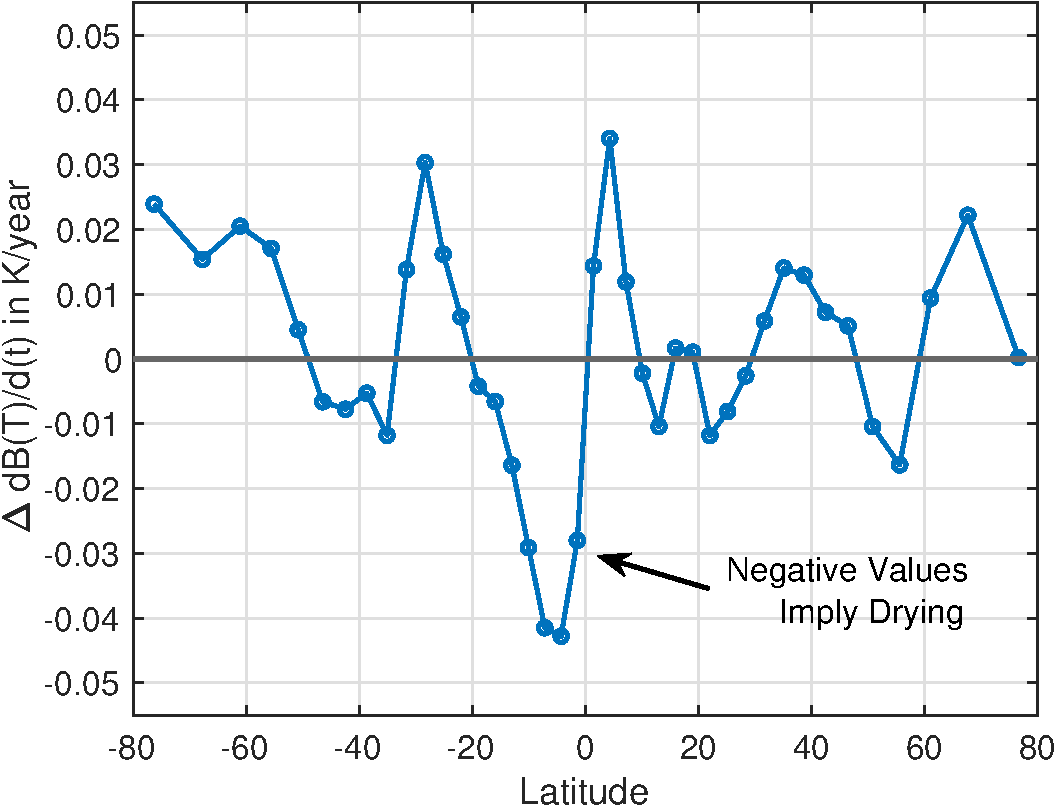
\includegraphics[width=0.7\linewidth]{./Figs/Pdf/drying_in_convective_regions_v2.pdf}
\end{center}

\vspace{-0.12in}
\begin{itemize}
\item \small Plotting latitude variability relative to the global mean ratio of dBT\textsubscript{T chan} vs dBT\textsubscript{Water chan}
\item \small Suggests relative drying in convective regions, moistening nearby
\item \small These results largely independent of any calibration drifts
\item \small These data are from "real?" climate trends, not ENSO-like proxies
\end{itemize}
\end{frame}

\begin{frame}[label={sec:orgb3e18be}]{Radiance Gridding: Minimize Cloud Variability}
\begin{itemize}
\item Radiance gridding combines clear + cloudy scenes
\item Clouds change slowly, but regional variability seen after 16 years
\item Want simple approaches to evaluating gridded radiances trends
\item Possible approach (suggested several years ago)
\begin{itemize}
\item Grid not ony mean radiance but:
\item Grid by rough measure of "clear"
\end{itemize}
\item Nominal approach
\begin{itemize}
\item Generate radiane anomaly
\item Separate 10\% hottest scenes in anomaly radiance, from colder (more cloudy) scenes.
\item Minimized cloud interferene for surface trending
\end{itemize}
\item Crude test done here
\begin{itemize}
\item Forget anomaly
\item Just trend 10\% hottest scenes in yearly gridded bins
\item Just one channel, 917 \wn
\end{itemize}
\end{itemize}
\end{frame}

\begin{frame}[label={sec:org6d74527}]{15-Year Global Trends: 10\% of Hottest Scenes (Desc node)}
\vspace{-0.15in}
\begin{columns}
\begin{column}{0.55\columnwidth}
\begin{block}{\scriptsize AIRS Trends (K/year)}
\vspace{-0.1in}
\begin{center}
\includegraphics[width=.9\linewidth]{./Figs/Png/desc_airs_hot_trend.png}
\end{center}

\vspace{-0.1in}
\small AIRS Global trend: 0.019K/year \\
\small AIRS Global std: 0.043K/year 
\end{block}
\end{column}

\begin{column}{0.55\columnwidth}
\begin{block}{\scriptsize ERA Surface Trends for \emph{these} Scenes}
\vspace{-0.1in}
\begin{center}
\includegraphics[width=.9\linewidth]{./Figs/Png/desc_era_hot_trend.png}
\end{center}


\vspace{-0.1in}
\small ERA Global trend: 0.019K/year \\
\small ERA Global std: 0.049K/year
\end{block}
\end{column}
\end{columns}

\begin{itemize}
\item \small Quite similar, no cloud patterns?
\item \small High cancellation of trends, but not to zero
\item \small Very simple, accuracy can be modeled
\end{itemize}
\end{frame}

\begin{frame}[label={sec:orgbdbf733}]{Compare Trends to Full ERA Sampling}
\vspace{-0.35in}
\begin{columns}
\begin{column}{0.55\columnwidth}
\begin{block}{\scriptsize AIRS Trends (K/year)}
\vspace{-0.1in}
\begin{center}
\includegraphics[width=0.9\linewidth]{./Figs/Png/desc_airs_hot_trend.png}
\end{center}
\end{block}
\end{column}

\begin{column}{0.55\columnwidth}
\begin{block}{\scriptsize ERA Surface Trends for \emph{these} Scenes}
\vspace{-0.1in}
\begin{center}
\includegraphics[width=0.9\linewidth]{./Figs/Png/desc_era_hot_trend.png}
\end{center}
\end{block}
\end{column}
\end{columns}



\begin{columns}
\begin{column}{0.55\columnwidth}
\begin{block}{\scriptsize Cloud Forcing Patterns (K)}
\vspace{-0.1in}
\begin{center}
\includegraphics[width=0.9\linewidth]{./cloud_forcing.png}
\end{center}]
\end{block}
\end{column}



\begin{column}{0.55\columnwidth}
\begin{block}{\scriptsize ERA Surface Trends (full Sampling)}
\vspace{-0.1in}
\begin{center}
\includegraphics[width=0.9\linewidth]{./Figs/Png/desc_era_fullsamp_trends.png}
\end{center}
\end{block}
\end{column}
\end{columns}
\end{frame}


\begin{frame}[label={sec:org0822d5d}]{Global Variability for This 10\% Hot Subset}
\vspace{-0.35in}
\begin{columns}
\begin{column}{0.55\columnwidth}
\begin{block}{\small AIRS Std (over time, in K)}
\vspace{-0.1in}
\begin{center}
\includegraphics[width=\linewidth]{./Figs/Png/desc_airs_hot_std.png}
\end{center}
\end{block}
\end{column}

\begin{column}{0.55\columnwidth}
\begin{block}{\small ERA Std (over time, in K)}
\vspace{-0.1in}
\begin{center}
\includegraphics[width=\linewidth]{./Figs/Png/desc_era_hot_std.png}
\end{center}
\end{block}
\end{column}
\end{columns}

\begin{itemize}
\item Quite similar!
\item No obvious cloud patterns?
\item High North polar variability
\item Just an example of what can be done without retrievals!
\end{itemize}
\end{frame}

\begin{frame}[label={sec:org4cfb38f}]{Global Trend in 902 \wn Channel: All Scenes}
\vspace{-0.1in}
\begin{center}
\includegraphics[width=0.7\linewidth]{./Figs/Pdf/bt902_global_trend_vs_time.pdf}
\end{center}

\vspace{-0.15in}

\begin{itemize}
\item \small Global average time series of 902 \wn channel with 2-year smoothing
\item \small Globally most of the trend took place in the last four years
\item \small It is now starting to turn around
\end{itemize}
\end{frame}

\begin{frame}[label={sec:orgd69b81c}]{Conclusions}
\begin{itemize}
\item Good progress in defining "good" channels for CHIRP
\item CHIRP radiometric stablility evaluation on-going
\begin{itemize}
\item Need to examine time-dependence more carefully
\end{itemize}
\item CHIRP "L1c" product nearly ready for implementation (need AIRS L1c)
\item CHIRP gridded "L3" product being assessed
\begin{itemize}
\item Very valuable to have all scenes paired with re-analysis
\item Several type of gridding seem worthwhile (all sky, gridded by nominal \% clear)
\end{itemize}
\item OEM retrievals of T/Q zonal trends will continue with an emphasis on observation error co-variances and better all-sky cloudy jacobians
\end{itemize}
\end{frame}
\end{document}